\section{Five comparisons (C1--C5)}
\label{sec:designs}

The full analysis numbers five contrasts on the live harvest \parencite{maurya2025simulating}.
C1 holds scoring mode and varies identity mix.
C2 and C3 hold the arm and vary the instrument.
C4 crosses both factors and is not a headline.
C5 concatenates live cells; that concatenation is not a physical super-graph.
Each contrast is descriptive.
$N=1$ supplies point estimates only.
Exploratory rank tests in \texttt{COMPARISONS.md} are not treated as replicate inference.

\subsection{C1: same topology, H versus He, same mode}

C1 pairs \texttt{T2c\_H} with \texttt{T2c\_He}, and \texttt{T2d\_H} with \texttt{T2d\_He}.
\Cref{fig:c1,fig:c1d} and \Cref{tab:c1} report the topology split.

Cell-pooled same-mode $\Delta(\mathrm{He}-\mathrm{H})$ is $0.1549$ continuous (H $0.8643$ versus He $1.0192$) and $0.3986$ dual-discrete (H $1.6814$ versus He $2.0800$).
Topology-equal means do not flip the sign (continuous $0.1725$; dual-discrete $0.3974$).
He exceeds H on 4 of 8 topologies in continuous mode and on 8 of 8 in dual-discrete mode.
Continuous He$>$H is therefore not uniform: He is higher on small-world, echo chamber, polarised, and hierarchical graphs; H is higher on linear chain, ring, ER, and scale-free.

That pattern is not \enquote{hetero buffers firestorms}.
Collapsed H mixes conspiracy personas with scientists.
Collapsed He mixes conspiracy-heavy \texttt{mix\_00}/\texttt{mix\_01} with conspiracy-free \texttt{mix\_02}.
Dead He cells remain hatched after LLM calls.

\begin{figure}[t]
\centering
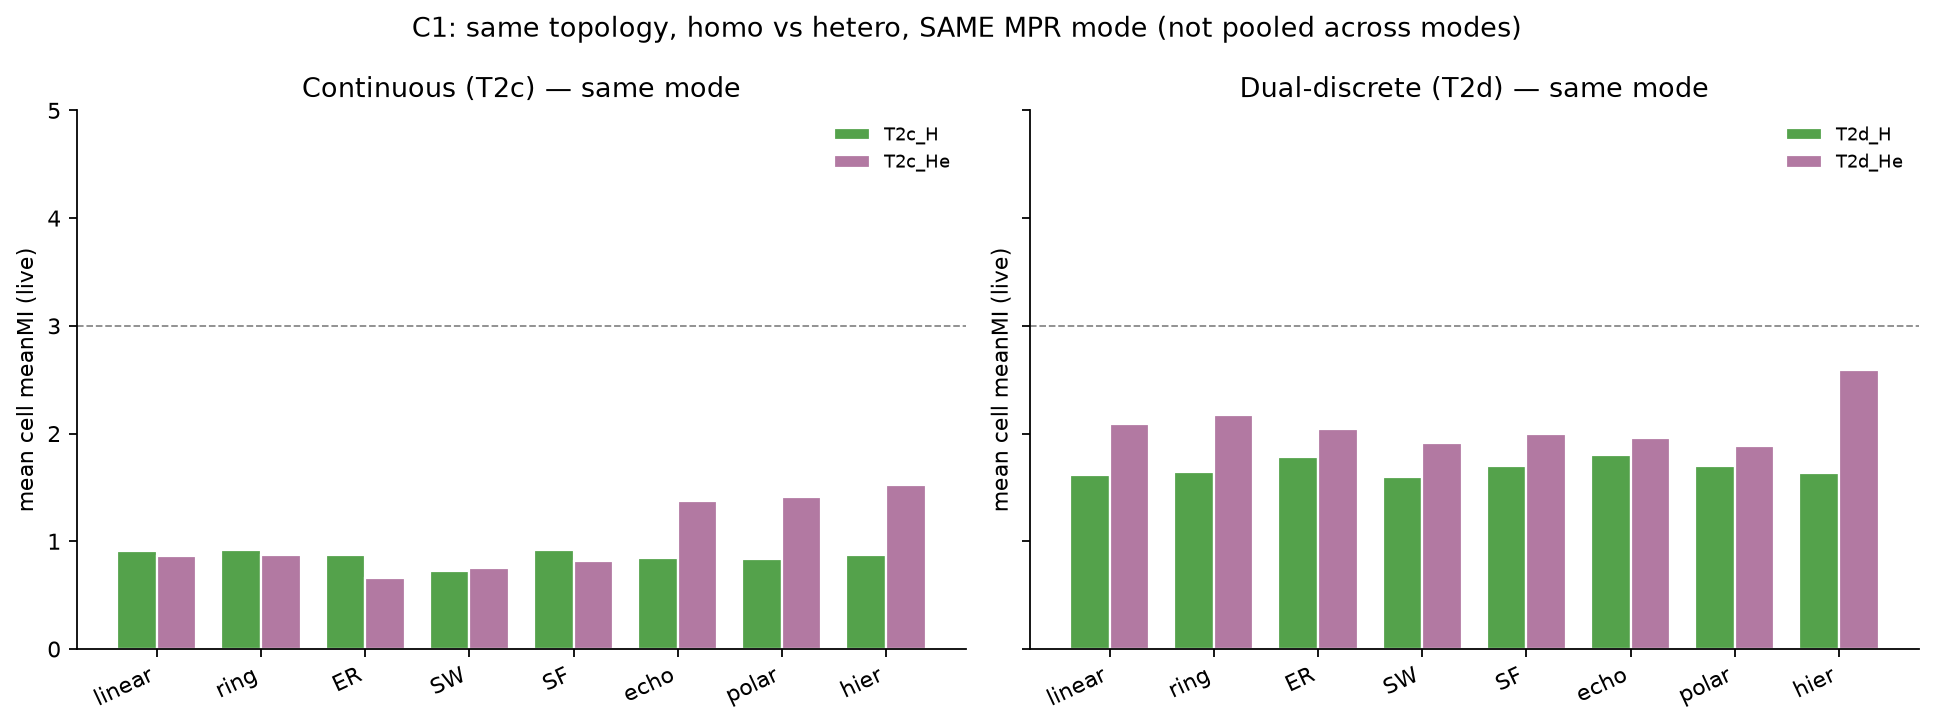
\includegraphics[width=\textwidth]{figures/fig01_c1_h_vs_he_same_mode.png}
\caption[C1 same-mode H vs He]{C1: same-mode H versus He by topology.
Left: continuous.
Right: dual-discrete.
The two panels are not averaged.
$N=1$.
Source: \texttt{fig01\_c1\_h\_vs\_he\_same\_mode.png}.}
\label{fig:c1}
\end{figure}

\begin{figure}[t]
\centering
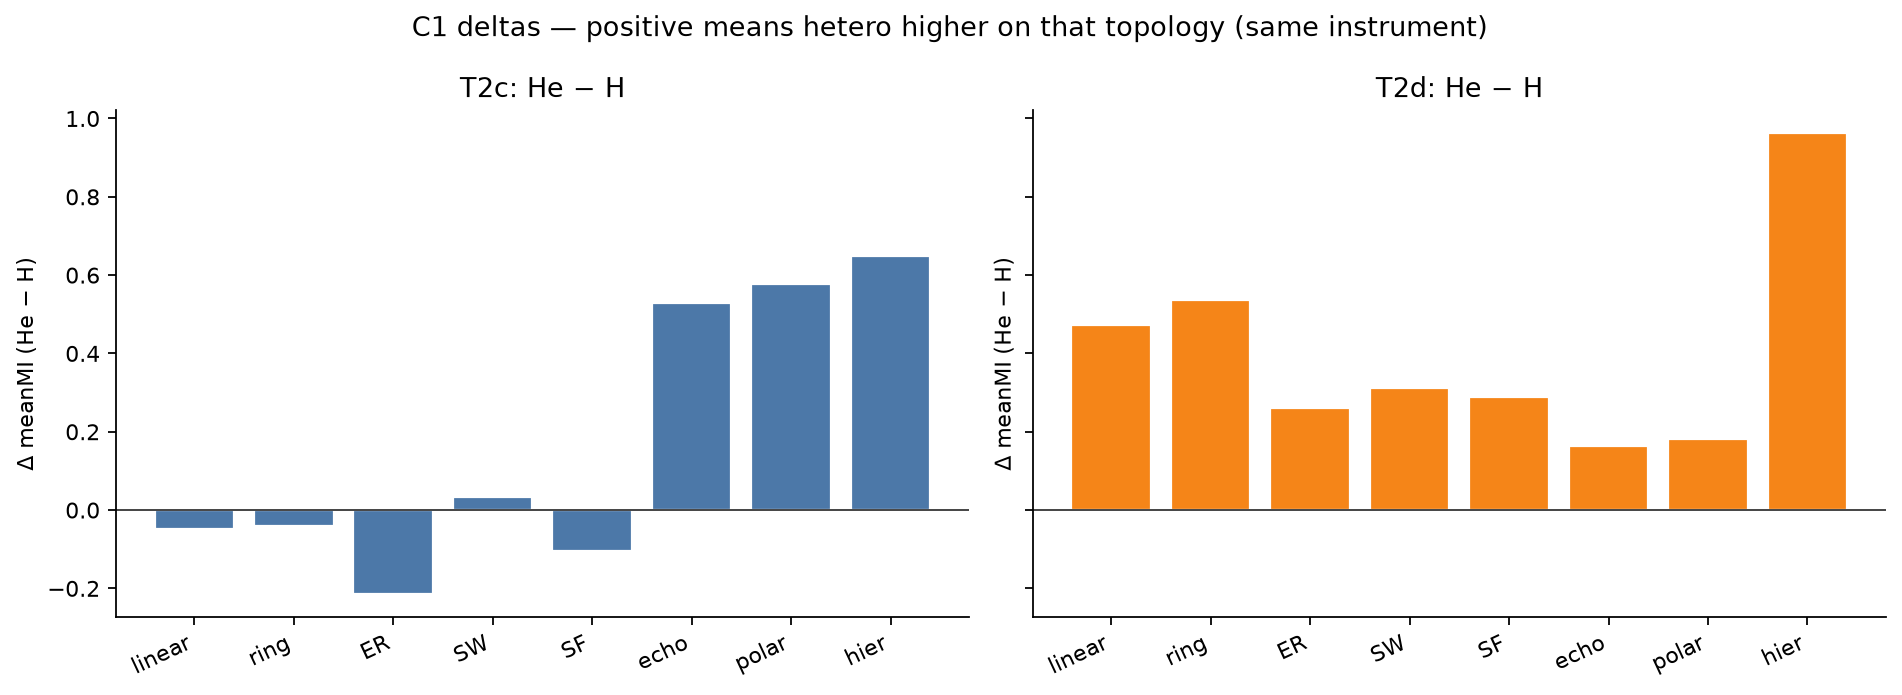
\includegraphics[width=\textwidth]{figures/fig02_c1_delta_he_minus_h.png}
\caption[C1 delta He minus H]{C1: $\Delta(\mathrm{He}-\mathrm{H})$ by topology, separately for each instrument.
Positive values mean He scored higher.
$N=1$.
Source: \texttt{fig02\_c1\_delta\_he\_minus\_h.png}.}
\label{fig:c1d}
\end{figure}

\begin{table}[t]
\centering
\caption[C1 same-mode topology means]{C1 live-cell mean \texttt{meanMI} by topology.
$\Delta$ is He minus H inside one instrument.}
\label{tab:c1}
\small
\begin{tabular}{lrrrrrr}
\toprule
Topology & T2c H & T2c He & $\Delta$ He$-$H & T2d H & T2d He & $\Delta$ He$-$H \\
\midrule
linear chain & 0.9129 & 0.8638 & $-0.0491$ & 1.6127 & 2.0852 & 0.4725 \\
ring & 0.9160 & 0.8760 & $-0.0400$ & 1.6402 & 2.1768 & 0.5366 \\
random ER & 0.8736 & 0.6593 & $-0.2143$ & 1.7809 & 2.0412 & 0.2602 \\
small world & 0.7215 & 0.7545 & 0.0330 & 1.5977 & 1.9096 & 0.3120 \\
scale-free & 0.9205 & 0.8157 & $-0.1048$ & 1.7034 & 1.9924 & 0.2890 \\
echo chamber & 0.8490 & 1.3775 & 0.5284 & 1.7984 & 1.9632 & 0.1647 \\
polarised & 0.8356 & 1.4137 & 0.5780 & 1.7005 & 1.8830 & 0.1825 \\
hierarchical & 0.8751 & 1.5242 & 0.6490 & 1.6315 & 2.5934 & 0.9618 \\
\bottomrule
\end{tabular}
\end{table}

\subsection{C2: homogeneous arm, different instruments}

C2 holds the homogeneous arm and compares \texttt{T2c\_H} with \texttt{T2d\_H}.
\Cref{tab:c2} reports the topology split.
Dual-discrete sits above continuous on 8 of 8 H topologies.
The mean topology $\Delta(\mathrm{disc}-\mathrm{cont})$ is $0.8201$.
Paired live cells (same topology $\times$ persona $\times$ article, both live) number 398; the median paired $\Delta$ is $0.8125$.
Cells dead on one side only were not filled with zero (T2c 80, T2d 82, both dead 16).

This gap is a scoring-mode difference.
It is not evidence that the dual campaign found more misinformation in a shared unit.
Dual gap on H live cells (discrete minus sidecar continuous on the same dual events) is $0.8804$.
That sidecar is not the T2c headline.

\begin{table}[t]
\centering
\caption[C2 homo T2c versus T2d]{C2 live-cell means.
$\Delta$ is dual-discrete minus continuous on homogeneous cells.
Dual gap is sidecar continuous on the same dual events, not the T2c headline.}
\label{tab:c2}
\scriptsize
\begin{tabular}{lrrrrrr}
\toprule
Topology & T2c H & T2d H & $\Delta$ & $n$ T2c & $n$ T2d & Dual gap \\
\midrule
linear chain & 0.9129 & 1.6127 & 0.6999 & 62 & 68 & 0.9672 \\
ring & 0.9160 & 1.6402 & 0.7242 & 65 & 61 & 0.8803 \\
random ER & 0.8736 & 1.7809 & 0.9073 & 57 & 56 & 0.9680 \\
small world & 0.7215 & 1.5977 & 0.8762 & 56 & 59 & 0.8255 \\
scale-free & 0.9205 & 1.7034 & 0.7829 & 60 & 57 & 0.8463 \\
echo chamber & 0.8490 & 1.7984 & 0.9494 & 63 & 61 & 0.8923 \\
polarised & 0.8356 & 1.7005 & 0.8649 & 65 & 57 & 0.8553 \\
hierarchical & 0.8751 & 1.6315 & 0.7564 & 52 & 59 & 0.7973 \\
\bottomrule
\end{tabular}
\end{table}

\subsection{C3: heterogeneous arm, different instruments}

C3 holds the heterogeneous arm and compares \texttt{T2c\_He} with \texttt{T2d\_He}.
\Cref{tab:c3} reports the topology split.
Dual-discrete sits above continuous on 8 of 8 He topologies.
The mean topology $\Delta(\mathrm{disc}-\mathrm{cont})$ is $1.0450$.
Paired live He cells number 198; the median paired $\Delta$ is $0.9778$.
Dual gap on He live cells is $1.1145$; agreement is $0.6174$.

\begin{table}[t]
\centering
\caption[C3 hetero T2c versus T2d]{C3 live-cell means.
$\Delta$ is dual-discrete minus continuous on heterogeneous cells.
Do not pool T2c with T2d.}
\label{tab:c3}
\scriptsize
\begin{tabular}{lrrrrrr}
\toprule
Topology & T2c He & T2d He & $\Delta$ & $n$ T2c & $n$ T2d & Dual gap \\
\midrule
linear chain & 0.8638 & 2.0852 & 1.2214 & 32 & 33 & 1.2960 \\
ring & 0.8760 & 2.1768 & 1.3008 & 33 & 33 & 1.3123 \\
random ER & 0.6593 & 2.0412 & 1.3818 & 29 & 29 & 1.1335 \\
small world & 0.7545 & 1.9096 & 1.1552 & 31 & 32 & 1.1049 \\
scale-free & 0.8157 & 1.9924 & 1.1767 & 30 & 29 & 1.1058 \\
echo chamber & 1.3775 & 1.9632 & 0.5857 & 32 & 30 & 0.8830 \\
polarised & 1.4137 & 1.8830 & 0.4693 & 25 & 26 & 0.8784 \\
hierarchical & 1.5242 & 2.5934 & 1.0692 & 26 & 28 & 1.1354 \\
\bottomrule
\end{tabular}
\end{table}

\Cref{fig:c23,fig:c23p} show C2 and C3 together.
The two instruments remain separate leagues.

\begin{figure}[t]
\centering
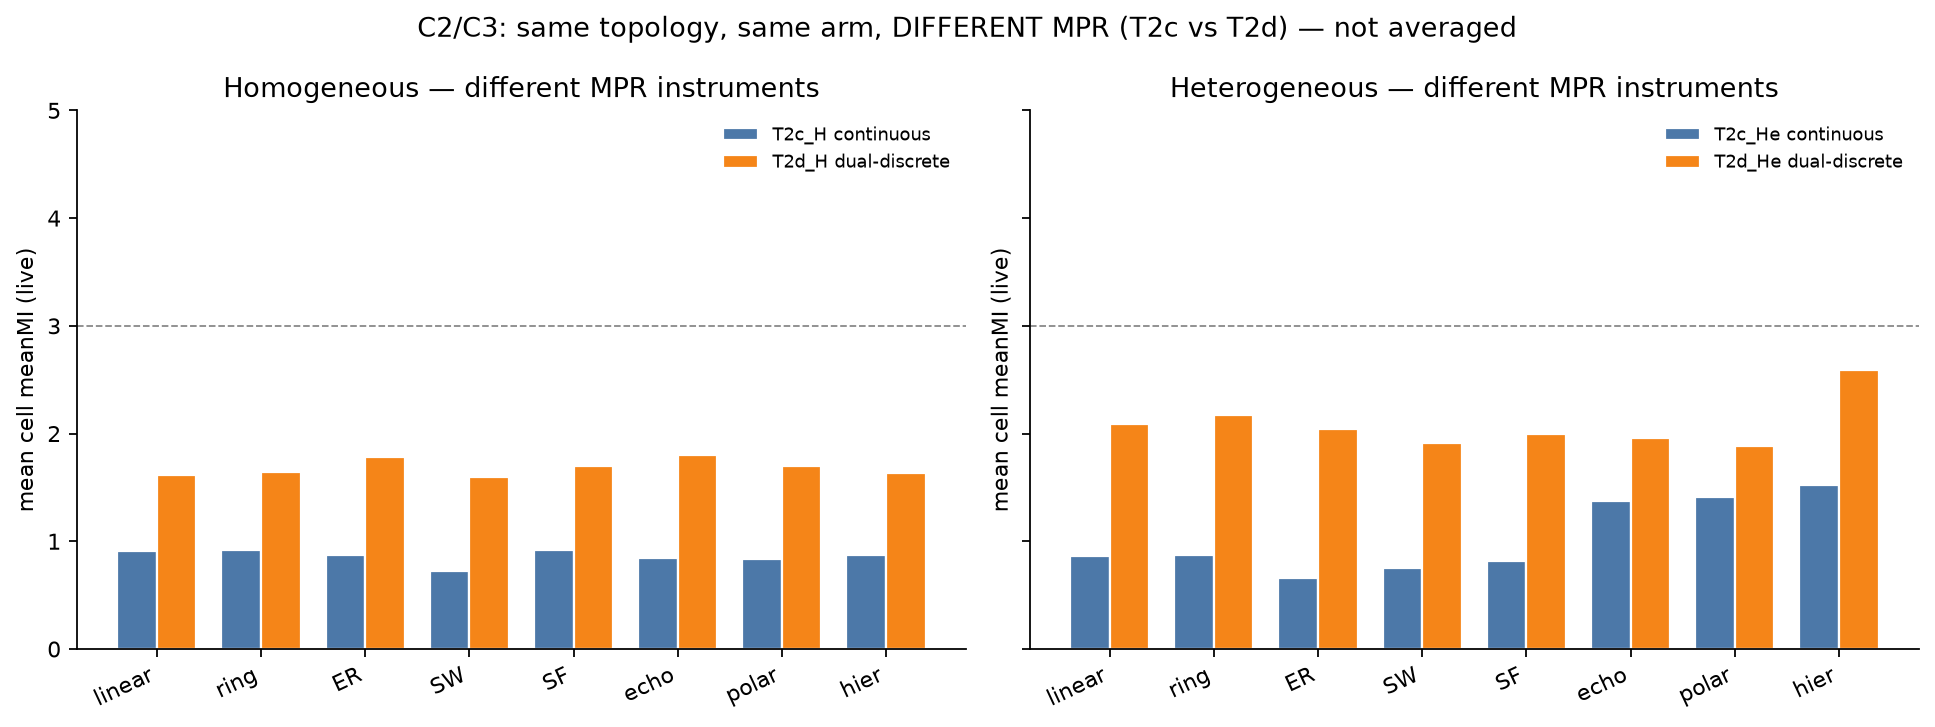
\includegraphics[width=\textwidth]{figures/fig03_c2_c3_same_arm_different_mpr.png}
\caption[C2 and C3 same-arm different MPR]{C2 and C3: T2c versus T2d within H and within He.
Dual-discrete sits above continuous on every topology in both arms.
$N=1$.
Source: \texttt{fig03\_c2\_c3\_same\_arm\_different\_mpr.png}.}
\label{fig:c23}
\end{figure}

\begin{figure}[t]
\centering
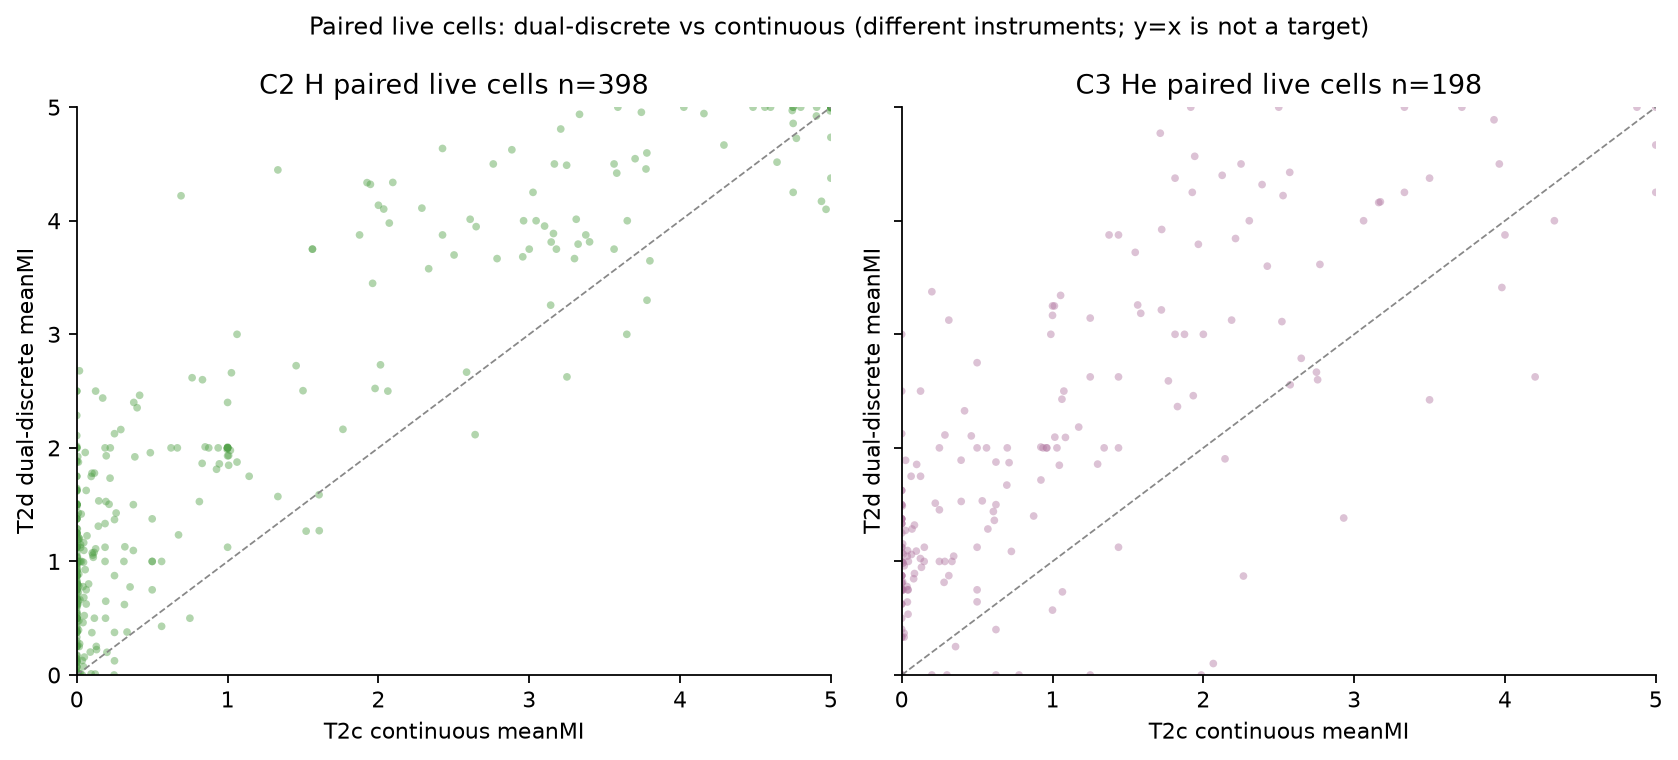
\includegraphics[width=\textwidth]{figures/fig04_c2_c3_paired_scatter.png}
\caption[C2 and C3 paired live cells]{Paired live cells, T2c versus T2d, for homogeneous and heterogeneous arms.
Points off the diagonal are instrument disagreement, not a third \MPR{}.
$N=1$.
Source: \texttt{fig04\_c2\_c3\_paired\_scatter.png}.}
\label{fig:c23p}
\end{figure}

\subsection{C4: cross-mode, two factors at once}

C4 pairs \texttt{T2c\_H} with \texttt{T2d\_He}, and \texttt{T2d\_H} with \texttt{T2c\_He}.
The table is labelled and unpooled.
No C4 headline is formed by averaging the two cross-mode deltas or by averaging discrete with continuous.

Mean topology $\Delta(\mathrm{T2d\_He}-\mathrm{T2c\_H})$ is $1.2176$.
That contrast mixes a higher-scoring instrument with the He composition mix.
It is not an identity effect.
Mean topology $\Delta(\mathrm{T2c\_He}-\mathrm{T2d\_H})$ is $-0.6476$.
Signs reverse because the scoring-mode gap is large.
\Cref{fig:c4} is the reason C4 must stay unpooled.

\begin{figure}[t]
\centering
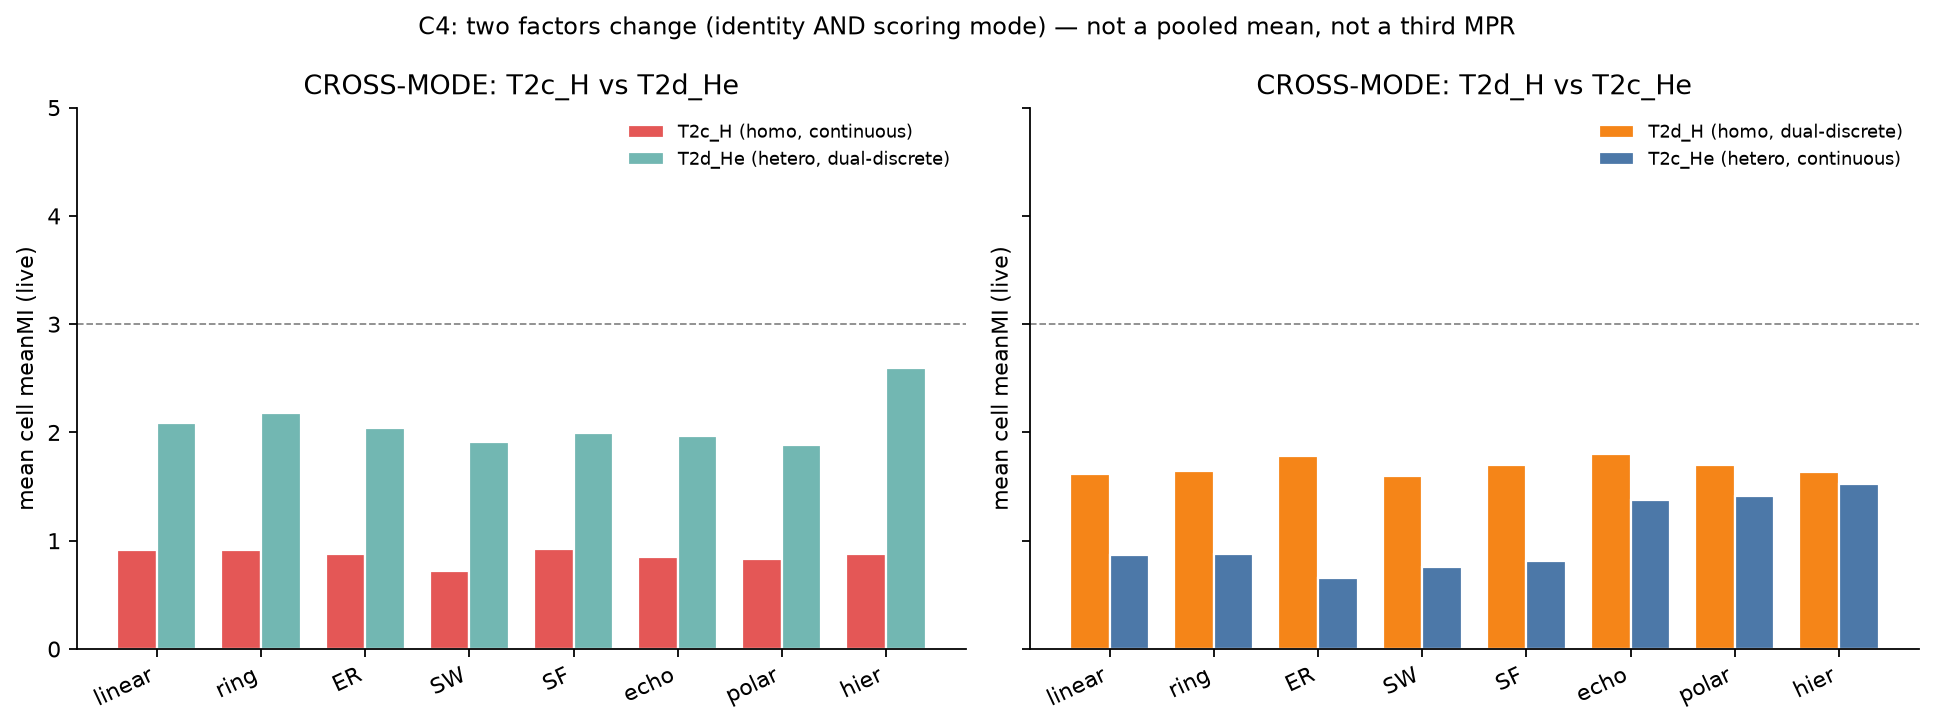
\includegraphics[width=\textwidth]{figures/fig05_c4_cross_mode.png}
\caption[C4 cross-mode]{C4: cross-mode two-factor table.
The two pairings are not averaged into a third \MPR{}.
$N=1$.
Source: \texttt{fig05\_c4\_cross\_mode.png}.}
\label{fig:c4}
\end{figure}

\begin{table}[t]
\centering
\caption[C4 cross-mode topology means]{C4 live-cell means.
The two $\Delta$ columns use different instrument pairings.}
\label{tab:c4}
\small
\begin{tabular}{lrrrrrr}
\toprule
Topology & T2c H & T2d He & $\Delta$ & T2d H & T2c He & $\Delta$ \\
\midrule
linear chain & 0.9129 & 2.0852 & 1.1724 & 1.6127 & 0.8638 & $-0.7489$ \\
ring & 0.9160 & 2.1768 & 1.2608 & 1.6402 & 0.8760 & $-0.7642$ \\
random ER & 0.8736 & 2.0412 & 1.1675 & 1.7809 & 0.6593 & $-1.1216$ \\
small world & 0.7215 & 1.9096 & 1.1881 & 1.5977 & 0.7545 & $-0.8432$ \\
scale-free & 0.9205 & 1.9924 & 1.0719 & 1.7034 & 0.8157 & $-0.8877$ \\
echo chamber & 0.8490 & 1.9632 & 1.1141 & 1.7984 & 1.3775 & $-0.4209$ \\
polarised & 0.8356 & 1.8830 & 1.0474 & 1.7005 & 1.4137 & $-0.2868$ \\
hierarchical & 0.8751 & 2.5934 & 1.7182 & 1.6315 & 1.5242 & $-0.1074$ \\
\bottomrule
\end{tabular}
\end{table}

Article valence is a secondary cut, not a sixth comparison.
\Cref{fig:valh,fig:valhe} show H and He article means on each instrument.
Chemtrails exceeds SCoPEx in the article collapse on both arms and both instruments.
The contrast still confounds topic, frame, and prior conspiracy fit.

\begin{figure}[t]
\centering
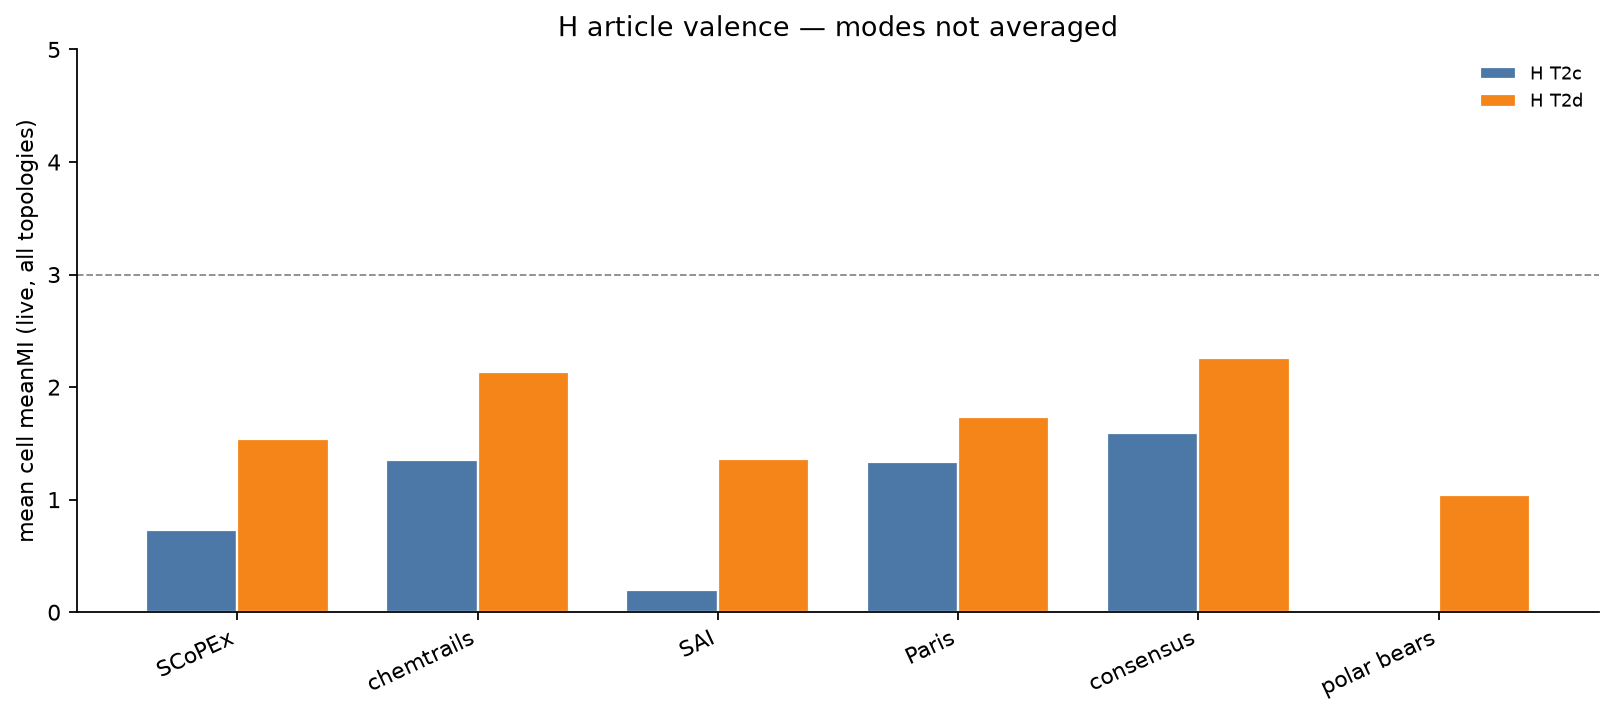
\includegraphics[width=0.92\textwidth]{figures/fig21_article_valence_h.png}
\caption[H article valence]{Homogeneous article (valence) collapse, discrete versus continuous.
Articles are a factor, not statistical replicates.
$N=1$.
Source: \texttt{fig21\_article\_valence\_h.png}.}
\label{fig:valh}
\end{figure}

\begin{figure}[t]
\centering
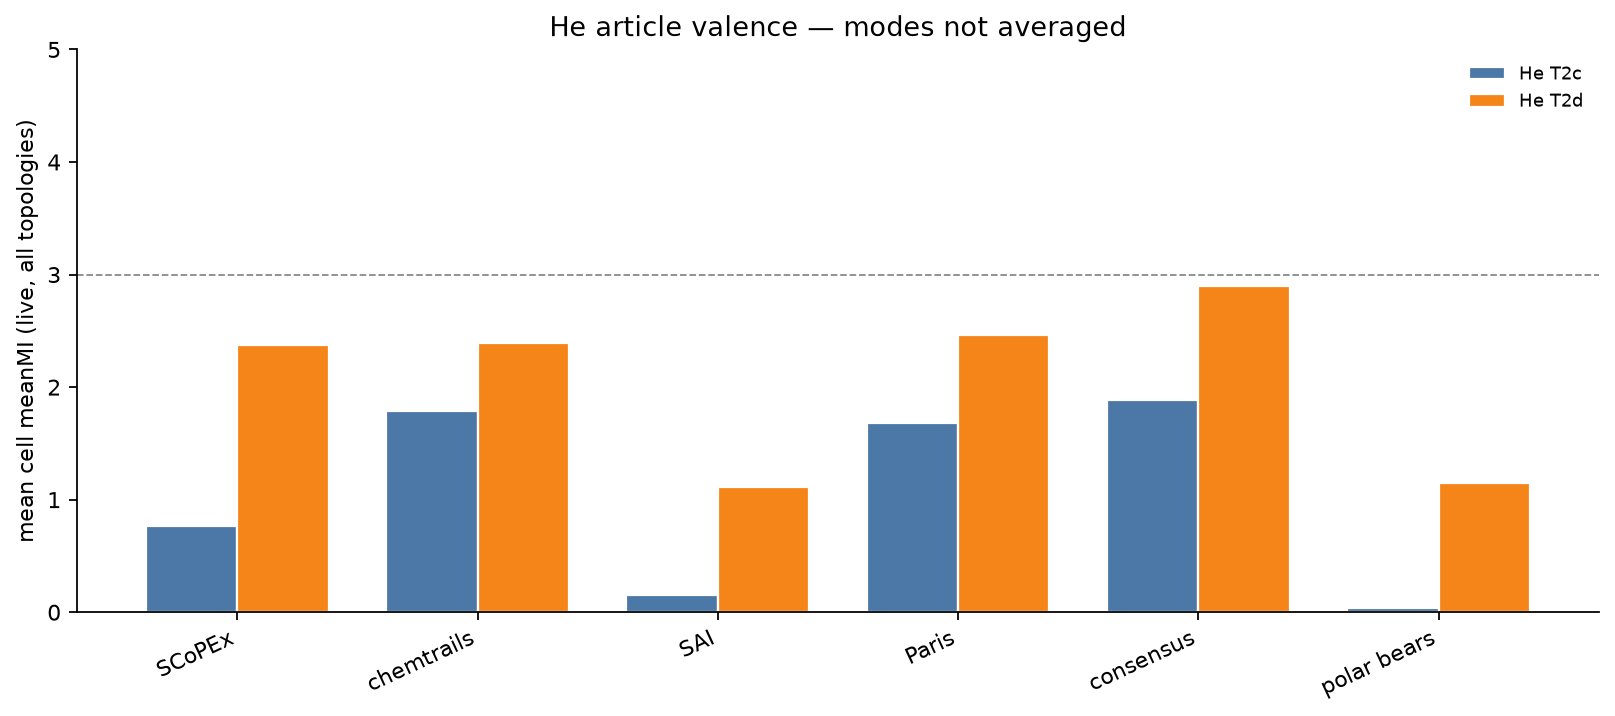
\includegraphics[width=0.92\textwidth]{figures/fig22_article_valence_he.png}
\caption[He article valence]{Heterogeneous article (valence) collapse, discrete versus continuous.
$N=1$.
Source: \texttt{fig22\_article\_valence\_he.png}.}
\label{fig:valhe}
\end{figure}
